\documentclass[11pt, leqno]{article}
\usepackage{amsmath}
\usepackage{amsfonts}
\usepackage{amssymb}
\usepackage{graphicx}
%american mathematical society - AMS 

\addtolength{\topmargin}{-.875in}
\addtolength{\textheight}{1.75in}

\usepackage{listings}
\lstset{
basicstyle=\small\ttfamily,
columns=flexible,
breaklines=true
}

\usepackage{enumerate}

\usepackage{wrapfig}
\usepackage{subfig}

\oddsidemargin = 0in
\textwidth=6.5in

\begin{document}


\begin{center}
\textbf{\large{Astronomy 345 Homework \#11 }} \\
By:Johnny Minor 
\end{center}

\begin{figure}[h!]
    \centering
    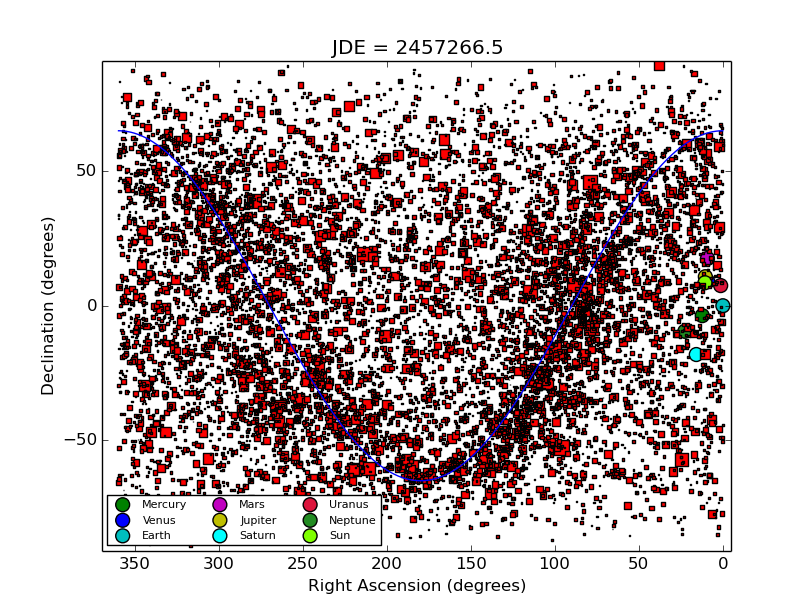
\includegraphics[width=\textwidth]{sept_1_2015_jde_2457266.png}
    \caption{Star plot for September 1st 2015}
    \label{fig:september1}
\end{figure}

\bigskip 

\begin{figure}[h!]
    \centering
    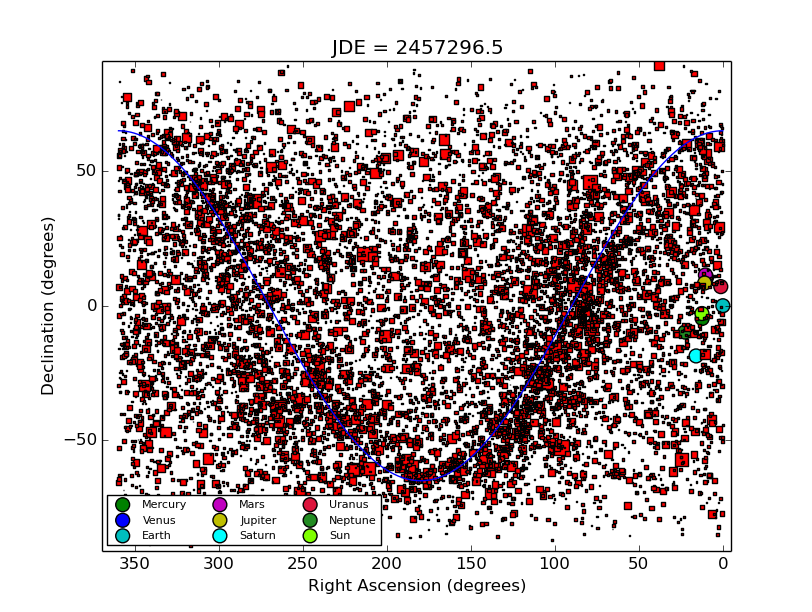
\includegraphics[width=\textwidth]{oct_1_2015_jde_2457296.png}
    \caption{Star plot for October 1st 2015}
    \label{fig:october1}
\end{figure}

\begin{figure}[h!]
    \centering
    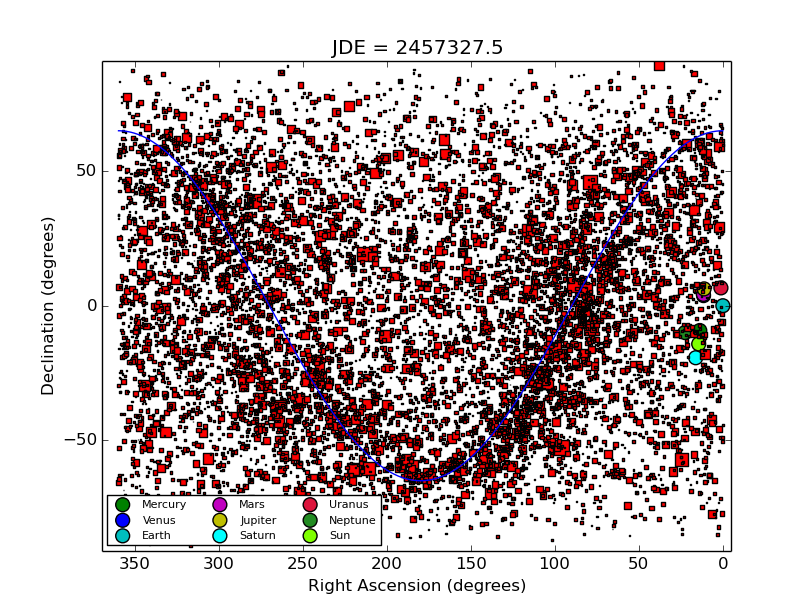
\includegraphics[width=\textwidth]{nov_1_2015_jde_jde_2457327.png}
    \caption{Star plot for November 1st 2015}
    \label{fig:november1}
\end{figure}






\end{document}